\documentclass[11pt]{article}
\usepackage{classTools}
\usepackage{algorithm}
\usepackage{algorithmic}

\begin{document}

% To include a problems set header, use the psHeader command
\psHeader{6}{Wed Oct. 30, 2024 (11:59pm)}

\textbf{Your name: Roshen Chatwal}

\textbf{Collaborators: Yaying Li, Raunak Daga, ChatGPT (for latex and learning some concepts)}

\textbf{No. of late days used on previous psets: approx 2 I think (around 27 hours total)}

\textbf{No. of late days used after including this pset: same }

The purpose of this problem set is practice proving optimality and efficiency of a greedy algorithm, practice modelling problems using graphs, reinforce understanding of the matching algorithm covered we learned, and think about ethical issues raised when modelling real-world problems for algorithmic solution.

\begin{enumerate}
    \item (Greedy Coloring for Interval Scheduling) The IntervalScheduling-Optimization problem we studied in class finds the largest group of nonintersecting intervals. 
    In many applications, it is also natural to consider the \emph{coloring} version of the problem, where we want to partition the input intervals into as few groups as possible so that each group is nonintersecting.
 
    In this problem, you will prove that Greedy Coloring in order of \emph{increasing start time} gives optimal coloring for interval scheduling. (Note the contrast with the \emph{increasing finish time} ordering we used for the version studied in class. It is a common phenomenon that different orderings are better for coloring vs. independent-set problems; for example, decreasing vertex degree is a good heuristic for greedy coloring of general graphs, while increasing vertex degree is a good heuristic for independent set.) Let \( x=(x_0,\ldots,x_{n-1}) \) be an instance of IntervalScheduling, where each \( x_i \) is an interval \([a_i,b_i]\) with \( a_i,b_i\in \mathbb{Q} \). Let \( k \) be the maximum number of input intervals that contain any value \( t\in \mathbb{Q} \). That is,
    \[
    k = \max_{t\in \mathbb{Q}} |\{ i\in [n] : t\in x_i\}|.
    \]

    \begin{enumerate}
        \item Prove that every proper coloring for Interval Scheduling uses at least \( k \) colors. \\

        \textbf{Proof by Contradiction:} 

        Assume, for contradiction, that there exists a proper coloring of the intervals using fewer than \( k \) colors.

        \textbf{Contradiction Argument:}

        By the definition of \( k \), there exists a time \( t \) at which \( k \) intervals overlap. For these intervals to be properly colored, each must have a distinct color because they all overlap at time \( t \). However, with fewer than \( k \) colors, it is impossible to assign distinct colors to \( k \) intervals, as this would require at least \( k \) unique colors.

        \textbf{Conclusion:}

        This contradiction implies that our assumption is false. Therefore, every proper coloring for Interval Scheduling requires at least \( k \) colors. \(\text{QED}\). \\

        \item Show that the Greedy Coloring in order of \emph{increasing start time} uses at most \( k \) colors. (To develop your intuition, carry out the algorithm on a few examples.) \\

        Let's take a look at a key condition for assigning colors via Greedy Coloring: $f(v_i) = \min \left\{ c \in \mathbb{N} : c \neq f(v_j) \, \forall j < i \text{ s.t. } \{v_i, v_j\} \in E \right\}.$ \\
        
        Greedy Coloring in order of \textit{increasing start time} upper bounds the number of colors used at $k$ due to the chronological order of vertices visited by start time. The only mechanism in which a new color will be assigned to an interval $x_i$ is when the start time $a_i \leq b_{j}$, where $b_{j}$ is the end time of every interval $x_{j}$ where $j < i$. This means that when iterating over our all the intervals sorted chronologically by start time, we only assign a new color when the current interval's start time is earlier than all of the preceding intervals' end times. This will occur at most $k$ times because that's the maximum number of intervals that all mutually contain the same time $t$ per the definition of $k$, meaning that maximum interval overlap won't be detected more than $k$ times. Since maximum overlap won't be detected more than $k$ times, no more than $k$ colors will be assigned because the detection of $a_i \leq b_{j}$, where $b_{j}$ is the end time of every interval $x_{j}$ where $j < i$, will happen at most $k$ times.  \\

        Ordering the intervals by \textit{increasing start time} makes color assignment much easier because the algorithm solely needs to compare the current interval's start time to each of the previous intervals' end times to detect conflict. Once $k$ colors are assigned, no more colors need to be assigned because when checking an interval's start time against the priors' end times, we know there will be at least one interval whose end time was prior to the current interval's start time (thereby allowing color(s) to be reused whereas coloring without ordering may have led to additional colorings due to the need for exhaustive perceived overlap checking that the Greedy algorithm, by design, usually doesn't dedicate time to exploring in depth). \\

        By my reasoning, I've shown that Greedy Coloring in order of \emph{increasing start time} uses at most \( k \) colors. \\

        \item Show that the Greedy Coloring in order of increasing start time can be implemented in time \( O(n\log n) \). \uline{Hints:}
        \begin{enumerate}
            \item Keep track of the end times of the most recently scheduled intervals assigned to each color, and use an appropriate data structure to ensure that you spend only \( O(\log k) \) rather than \( O(k) \) time per iteration, where \( k \) is the number of colors used.
            \item To make life easier for yourselves, you may instead implement a \emph{variant} of Greedy Coloring in which, at every step, you assign a vertex \emph{any color} not assigned to its neighbors that's also less than the largest color (as opposed to standard Greedy Coloring in which you assign the smallest color). \\
        \end{enumerate}
        
        I will provide an algorithm that implements Greedy coloring in order of increasing start time that can be implemented in time $O(n \log n)$. Let's say the $n$ intervals $x_i = (a_i, b_i)$, the input, are provided/converted in an array $A$ format for my algorithm's conceptual security. \\

\begin{center}
    \Large \textbf{THE ALGO}
\end{center} \\

\textbf{Preprocessing:} 

Sort the array $A$ of intervals using MergeSort, treating start times as keys, to get $A'$. This step helps us obtain an array of the same intervals, but in ascending order of start times. Initialize empty arrays $B$ and $C$ of size $n$ (we'll use them to track colors and store a list of dictionaries). Also, create an empty, size-augmented balanced AVL tree $T$. Additionally, set a variable $k = 0$ to be our counter for $k$ that updates when maximal conflicts are found (useful for assigning new colors). \\

\textbf{Processing:} 

Now it's time to apply the Greedy Coloring algorithm, iterating through the sorted interval array $A'$ in order from earliest to latest starting. 

\begin{itemize}
    \item For $i$ in range $(n)$:
    \begin{itemize}
        \item Define the variable $start_i = a_i$  for $a_i$ in $x_i$.
        \item Define the variable $end_i = b_i$  for $b_i$ in $x_i$.
        \item Define a temporary variable $lowest = \text{MINIMUM}(end_i)$ (queried on $T$).
        \item \textbf{If} $lowest \leq start_i$:
            \begin{itemize}
                \item Set $color_i = color'$, reusing the color $color'$ in the vertex $(lowest, color')$ of $T$.
                \item Assign $B[i] = color_i$.
                \item Form the $(K, V)$ tuple $(end_i, color_i)$.
                \item Query $\text{DELETE}(lowest)$ on $T$ and update $T$ using $\text{INSERT}((end_i, color_i))$ to ensure there's only a singular vertex with $color_i = color'$ that's altered to contain the ending time of the most recent interval assigned $color_i$.
            \end{itemize}
        \item \textbf{Else} (i.e., when $lowest > start_i$ or our MINIMUM query was done on an empty tree $T$):
            \begin{itemize}
                \item Set $color_i = k$.
                \item Assign $B[i] = color_i$.
                \item Form the $(K, V)$ tuple $(end_i, color_i)$.
                \item Update $T$ using $\text{INSERT}((end_i, color_i))$ to ensure a vertex with newly utilized $color_i$ as its value is present in $T$.
                \item Increment $k$ by 1.
            \end{itemize}
    \end{itemize}
\end{itemize} \\

\textbf{Post Processing:} 

Now we do some simple steps to obtain our colorings.

\begin{itemize}
    \item For $i$ in range($n$):
        \begin{itemize}
            \item Define a temporary variable $interval_i = A'[i]$. 
            \item Define a temporary variable $color_i = B[i]$.
            \item Create the tuple $(interval_i, color_i)$, which appears as $((a_i, b_i), color_i)$.
            \item Assign $C[i] = (interval_i, color_i)$.
        \end{itemize}
    \item \textbf{Return} $C$ (our list of intervals along with their coloring assignments).
\end{itemize} \\

\begin{center}
    \Large \textbf{Correctness and Runtime}
\end{center} \\

\textbf{Correctness:} 

The algorithm sorts the intervals in order of ascending start times and iterates over each interval (in chronological order). \\

In each iteration, the algorithm extracts the interval's starting and ending times, as well as the minimum ending time recorded in the tree T. \\

When the minimum ending time in the tree is $\leq$ the current interval's start time, it means that the current interval has no conflict with at least one interval. Thus it can share a color with one of those intervals, and to be concrete we let that interval be the one whose ending time and coloring are contained in the leftmost vertex of T. My algorithm correctly takes care of the color-sharing in this scenario by matching $x_i$'s color to that of $x_z$, where $z$ corresponds to the iteration in which the interval with the lowest ending time was represented in T. My algorithm also correctly handles updating the ending time of the vertex containing $color_i$ as requested to that of the most recent interval assigned $color_i$ (through deletion of the vertex $(end,color)$ where $end = lowest$ and insertion of the vertex $(end_i, color_i)$, assuming all the intervals have distinct end times). This updating is essential to my algorithm's correctness because it prevents overlap with future intervals using the same color. \\

Otherwise, when the minimum ending time in the tree DNE or is $>$ the current interval's start time, it means that the current interval must be assigned a new color. We know this is true because the ordering by ascending start times ensures that when a current interval conflicts with the earliest ending interval, it also conflicts with each of the intervals previously iterated over because all previous intervals have end times that extend beyond the start of the current interval. I handle this new color assignment correctly by assigning intervals that need a new color the value of $k$ that has been reached up to this point (initializing $k = 0$ allows the first interval we iterate over in A' to be correctly assigned color 0 once it's seen that MINIMUM(T) doesn't exist due to T's emptiness). To make sure T contains a vertex containing $color_i$ (which it doesn't yet when $color_i$ is a new color), I correctly update T by inserting the vertex $(end_i, color_i)$ to reflect the most recently observed ending time of the interval assigned $color_i$. Finally, incrementing $k$ up by one correctly ensures that the next time a new color is needed, it will be distinct from the prior ones and no larger than necessary. \\

Since the coloring assignments are correct for the reasons proven above, postprocessing is pretty intuitively correct. All we're doing is pairing an interval with its valid color assignment and returning a list of those $(interval_i, color_i)$ pairs as desired in a problem like coloring for IntervalScheduling. Thus, Greedy Coloring in order of \textit{increasing start time} has been implemented correctly since it will properly color intervals using up to (and no less than) $k$ colors and return a list of all the intervals along with their colorings. I'll prove that the runtime of my implementation fits our desired bounds next. \\

\textbf{Runtime Analysis:}

Preprocessing takes $O(n \log n + n + n + 1 + 1) = O(n \log n + 2n + 2) = O(n \log n)$ time asymptotically. \\

Processing takes $n \cdot O(1 + 1 + \log{k} + 1 + 1 + 1 + \log{k} + \log{k}) = n \cdot O(5 + 3 \log{k}) = O(n \log{k})$ time asymptotically. Every loop iteration uses a constant number of MIN queries and INSERT/DELETE operations on T, with them each taking $O(\log k)$ time due to properties of size-augmented balanced AVL trees and there being no more than $k$ vertices in a tree at any time (since we only keep vertices in T containing the end time of the most recent interval to be assigned to a corresponding color value and the algorithm won't use than $k$ colors for reasons proved in 1b). \\

Postprocessing takes $n \cdot O(1+1+1+1) + O(1) = n\cdot O(4) + O(1) = O(n)$ time. \\

Aggregating, I get that my algorithm takes $O(n \log n) + O(n \log{k}) + O(n) = O(n(\log n + \log{k}) + n) = O(n(\log n + \log n) + n) = O(2n \log n + n) = O(2n \log n) = O(n \log n)$ time, using the fact $k = O(n)$ since we can't have more colors assigned than the number of intervals we can assign them to. From this analysis and that above, I've proven that my correct Greedy Coloring algorithm in order of increasing start time can be implemented in time $O(n \log n)$.  \\

\end{enumerate}


    \item (Matching Algorithms) 
    One practical application of matching algorithms is planning logistics, like in the following example from (fictional) ridesharing service Lyber in (real) New York City's Times Square.  When a customer books a Lyber ride, the ride request is sent to a Lyber server and combined with others to create a schematic like the one drawn in the map below:

    \begin{figure}[H]
        \centering
        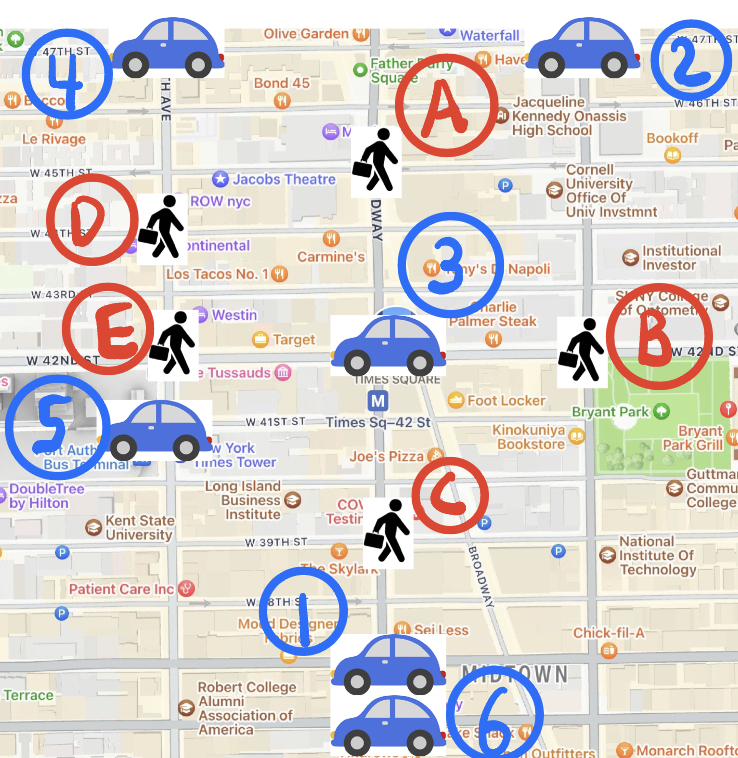
\includegraphics[width=0.87\textwidth]{fall2024/psets/ps6/NYC-map-zoomed-light.jpeg}
        \label{fig:travel_time_graph}
    \end{figure}

    Given a schematic like this, Lyber's goal is to serve as many customers (labeled A--E in the map) as possible, by assigning each one to a driver (labeled 1--6 in the map). For simplicity, each customer and driver is at an intersection, and assume driving between adjacent streets (vertical segment) takes 30 seconds, and driving between adjacent avenues (horizontal segments) takes 1 minute. However, the one twist is that they want to make sure that \textit{no customer is waiting for longer than 2 minutes}.  They also do not want to assign a driver to more than one customer at once, since serving a single customer can take more than 2 minutes.

    \begin{enumerate}
        \item To perform the assignment, they reduce to Maximum Matching in bipartite graphs.  Draw a bipartite graph corresponding to the drivers and customers in the map above.

    \begin{figure}[H]
        \centering
        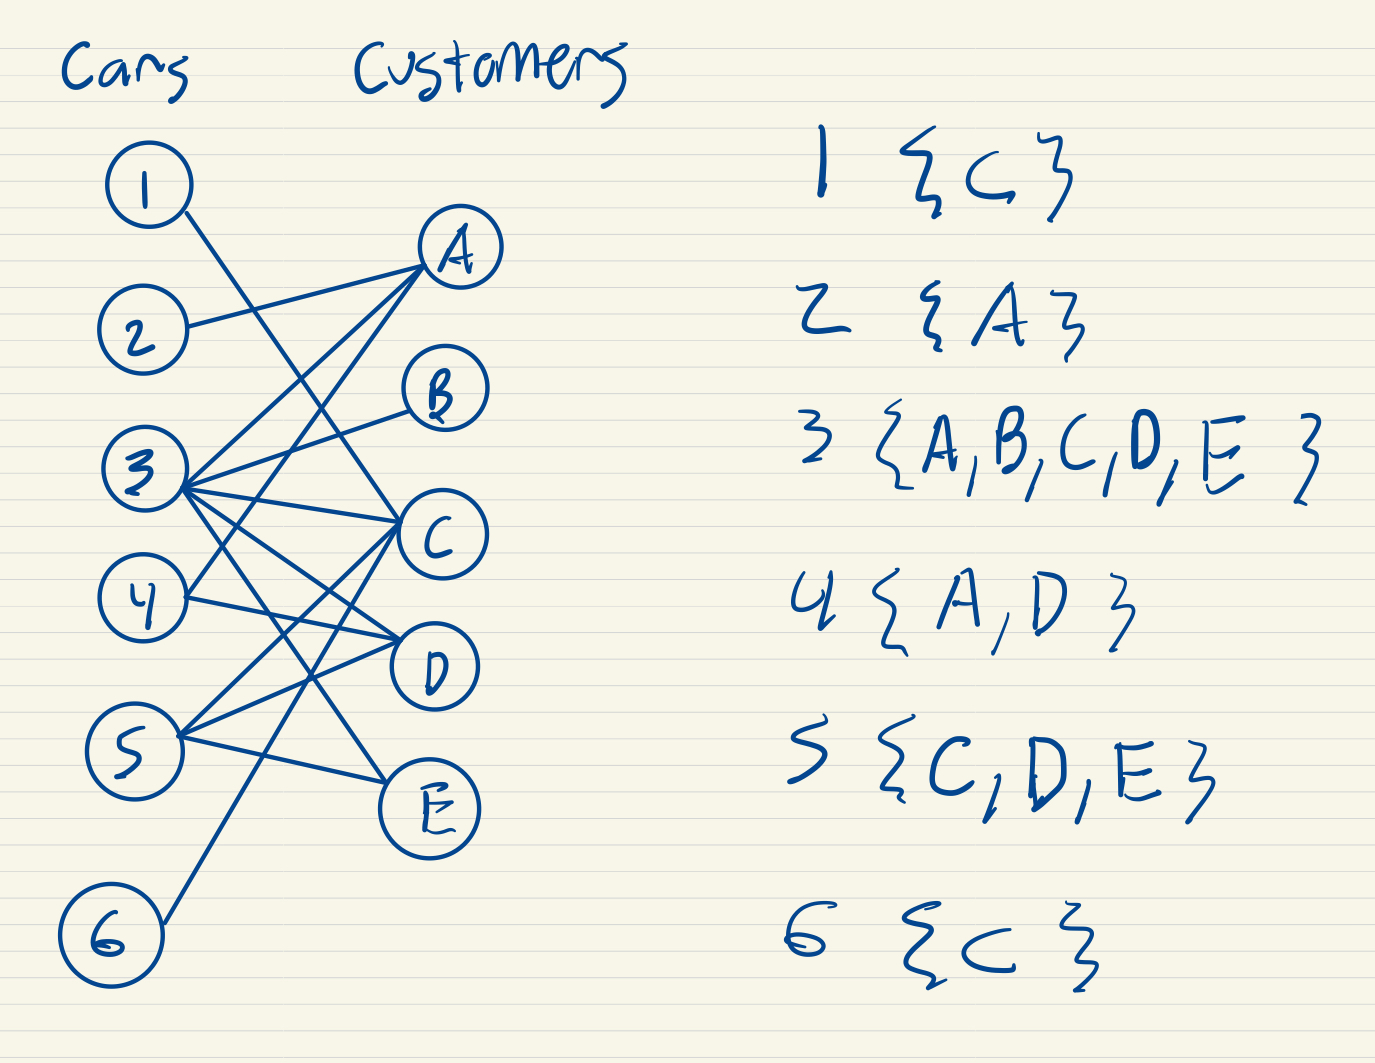
\includegraphics[width=0.75\linewidth]{42646.jpg}
        \caption{Bipartite graph w/ potential customers for each car listed}
        \label{fig:enter-label}
    \end{figure}
        
        \item The Lyber app first prioritizes customers on Broadway, so they initially assign customer $A$ to driver 3 and customer $C$ to driver 5. Using the algorithm from class, find a \textit{maximum matching} in the bipartite matching graph you've drawn, starting from the initial matching of $A$ to 3 and $C$ to 5. Draw pictures showing the sequence of matchings and augmenting paths you find. (No need to break down the steps of the algorithm to find the augmenting paths.) \\

I did this with the other algorithm covered in class in which we found shortest paths between unmatched vertices on a directed graph (unmatched cars point to unmatched customers, matched customers point to their car). I did this by using a point $x$ connected to the vertices in $U_0$ and $y$ connected to the vertices in $U_1$, finding a shortest walk between $x$ and $y$, and cutting out the start/end of the shortest walk to get a shortest walk between $U_0$ and $U_1$ (and thereby new edges to be added to the matching). It may not be the strategy you wanted but it one of "the algorithms from class" and I don't have the time to redo it lol. Here's my drawings, in which I use the shortest path to add to the alternating walk with respect to the current matching $M$ in my graph $G$. \\

\begin{figure}[H]
    \centering
    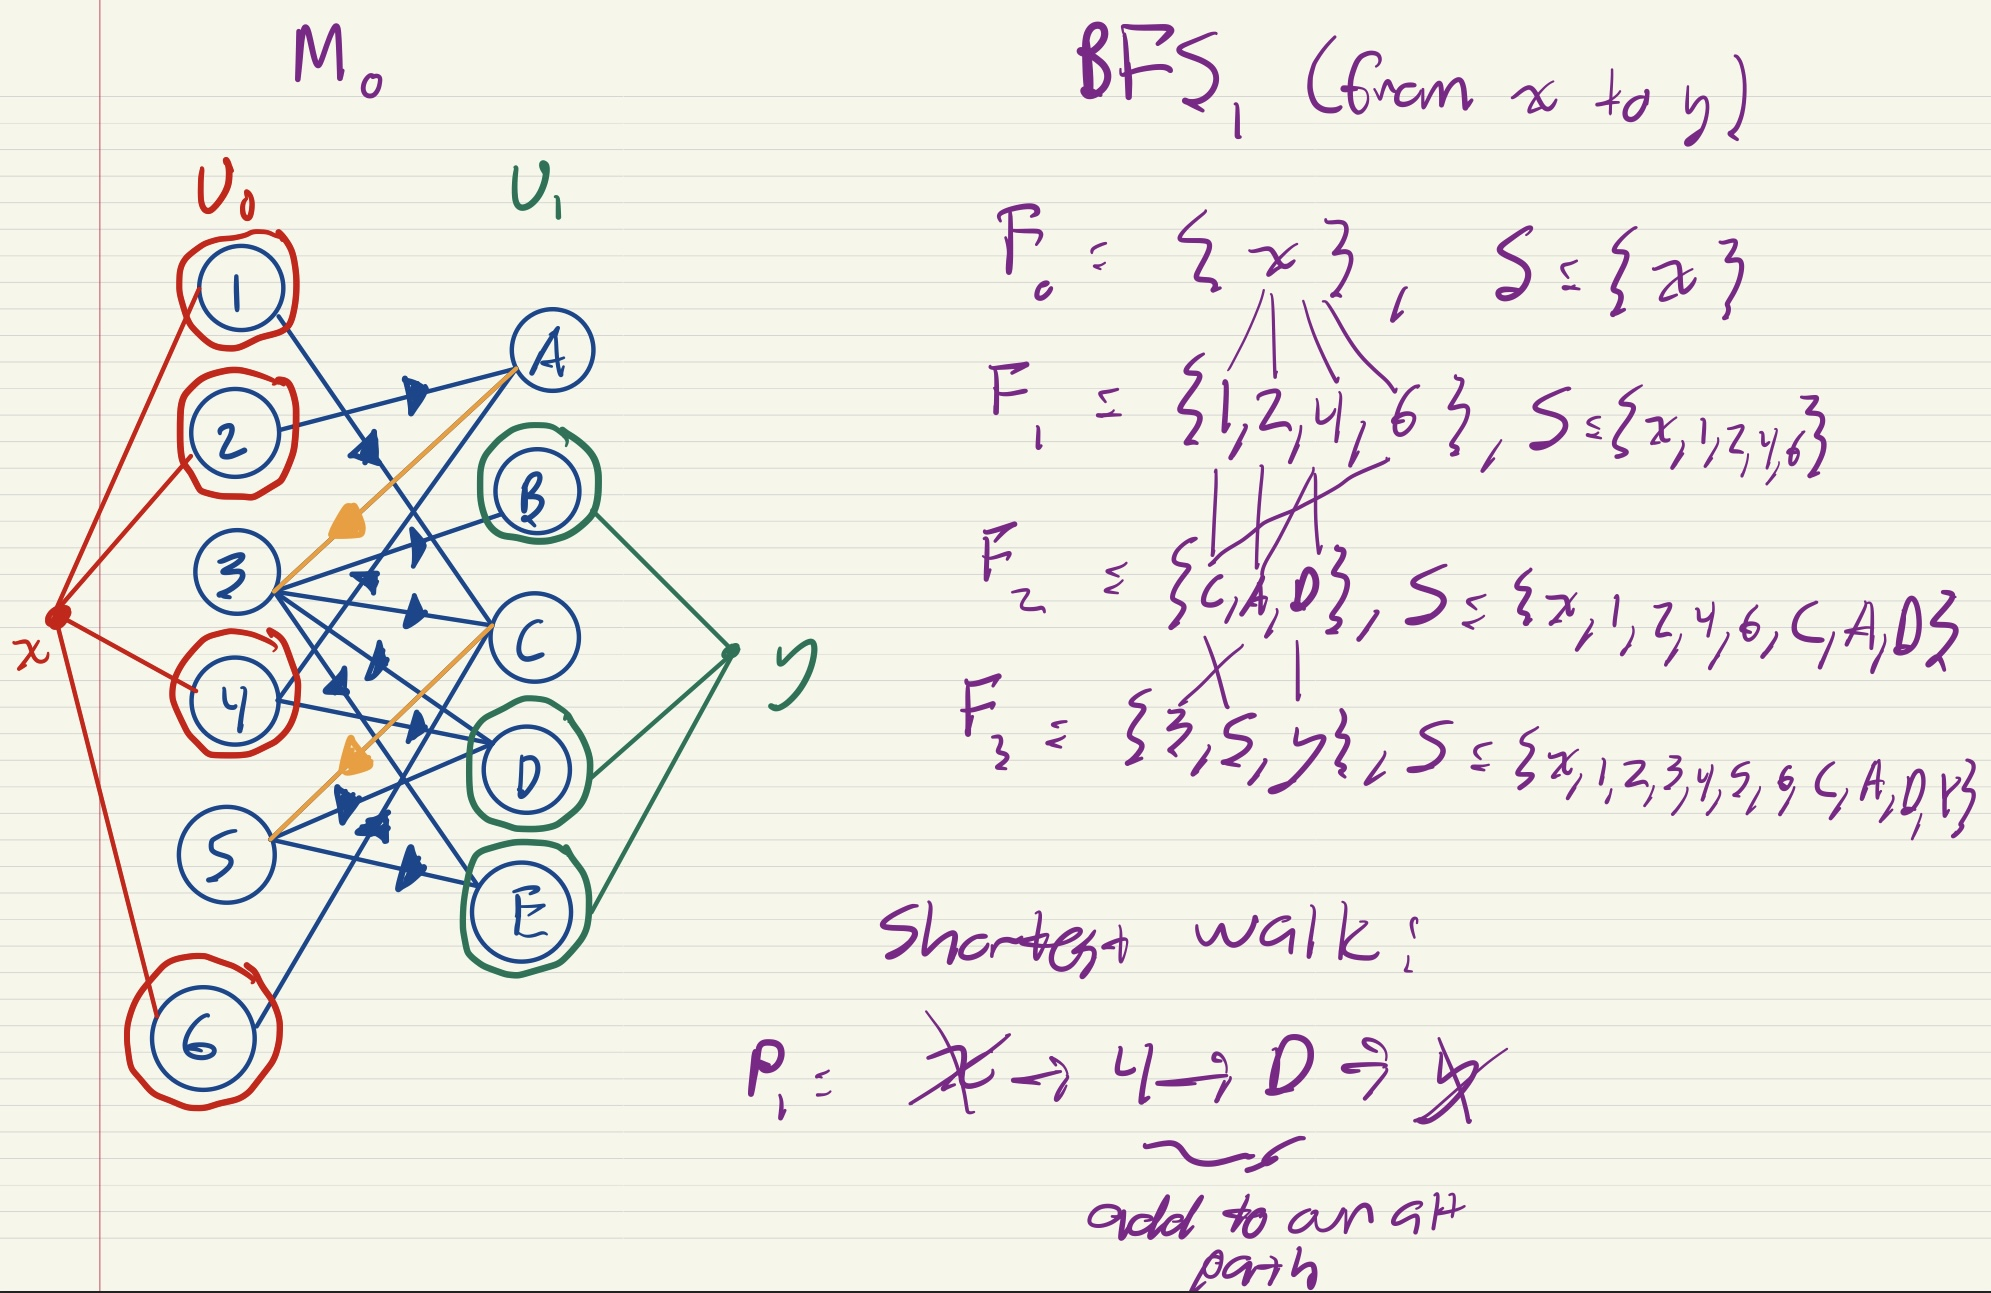
\includegraphics[width=0.75\linewidth]{IMG_0136.jpg}
    \caption{Original Matching, finding first shortestwalk}
    \label{fig:enter-label}
\end{figure}

\begin{figure}[H]
    \centering
    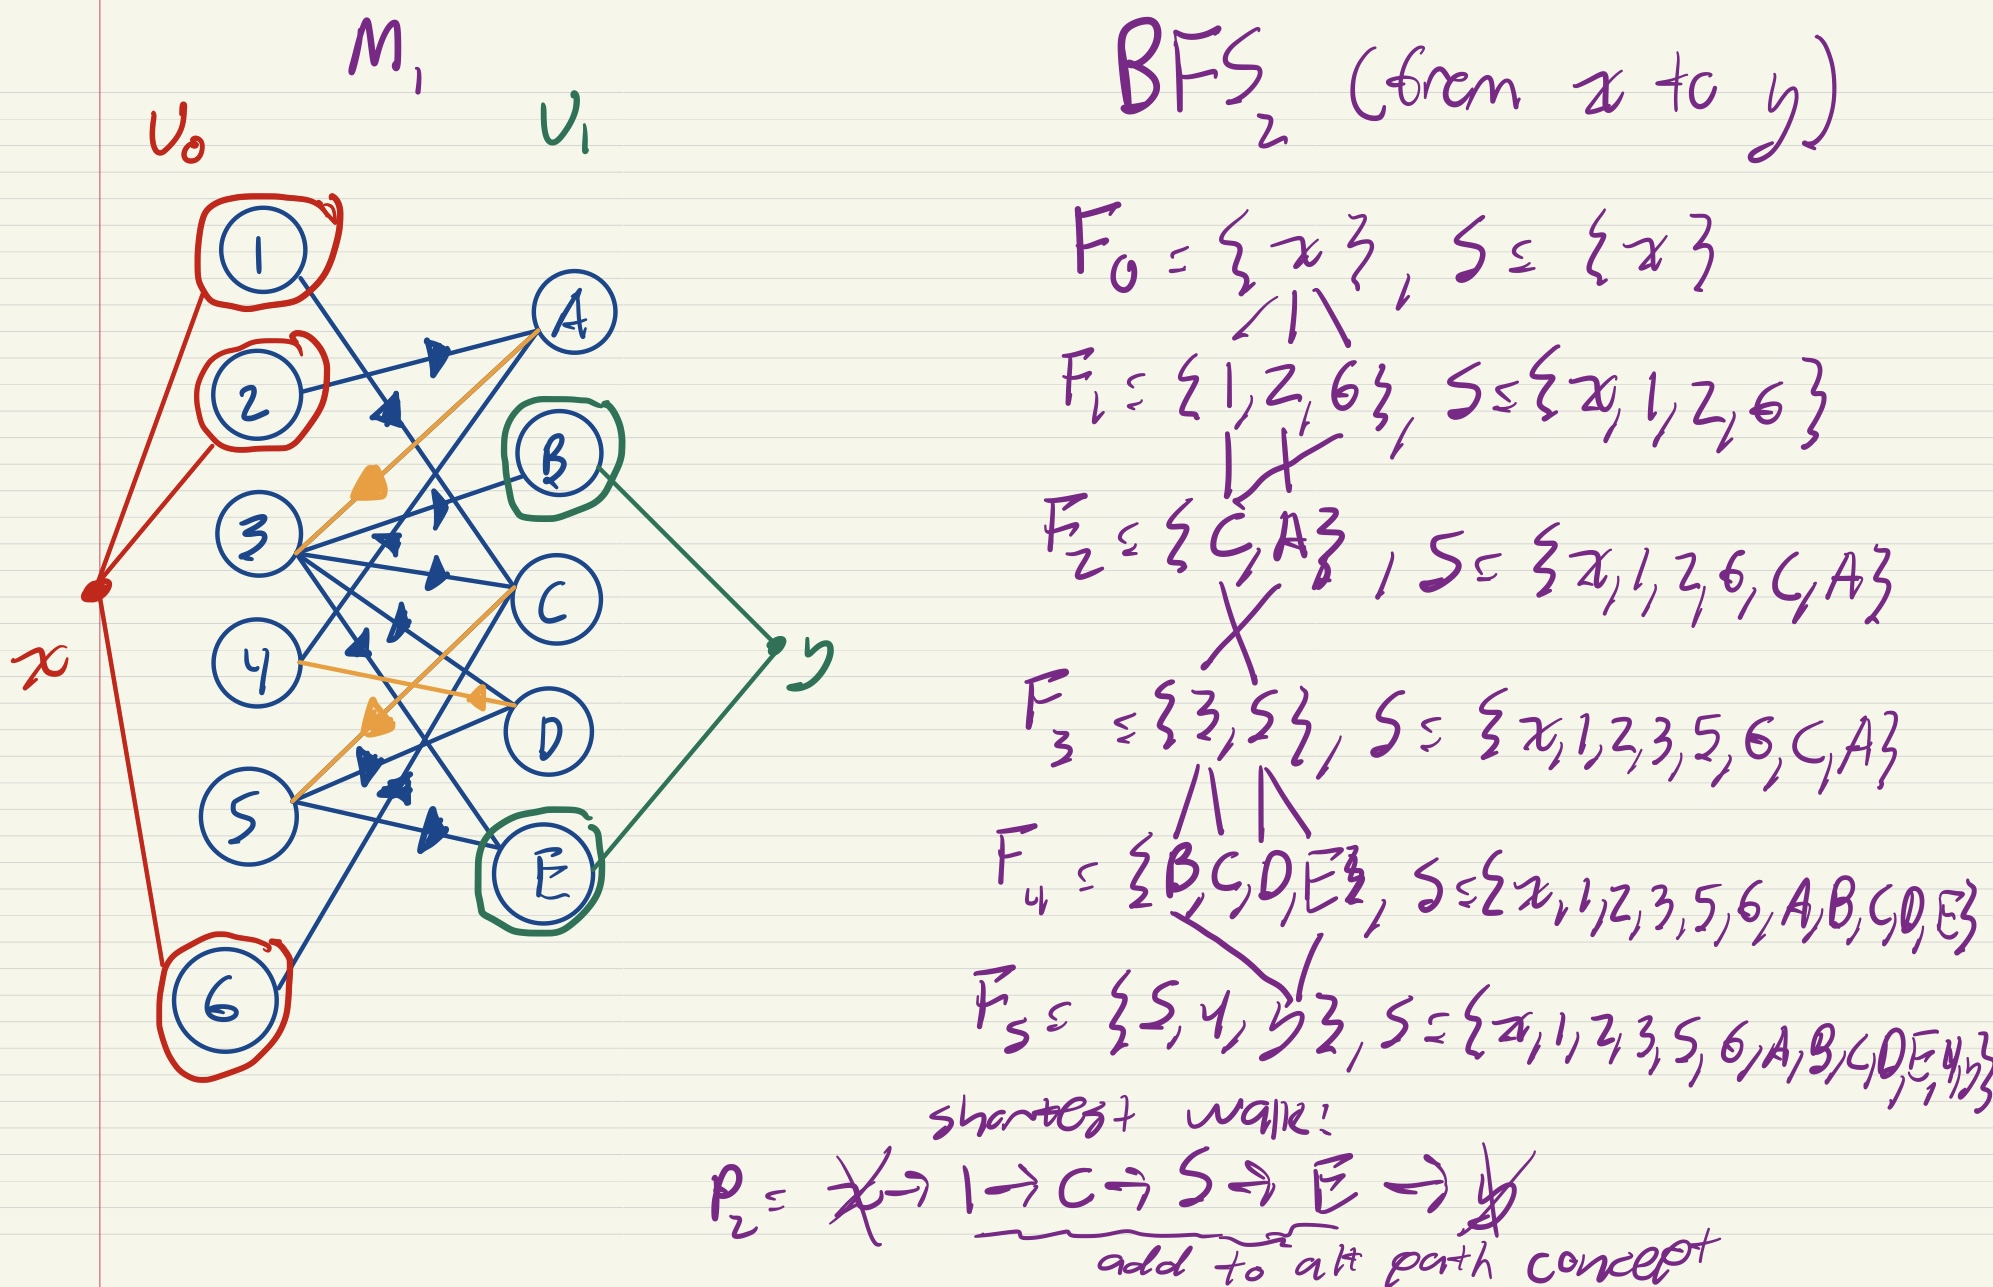
\includegraphics[width=0.75\linewidth]{IMG_0137.jpg}
    \caption{First matching update, finding second shortestwalk}
    \label{fig:enter-label}
\end{figure}

\begin{figure}[H]
    \centering
    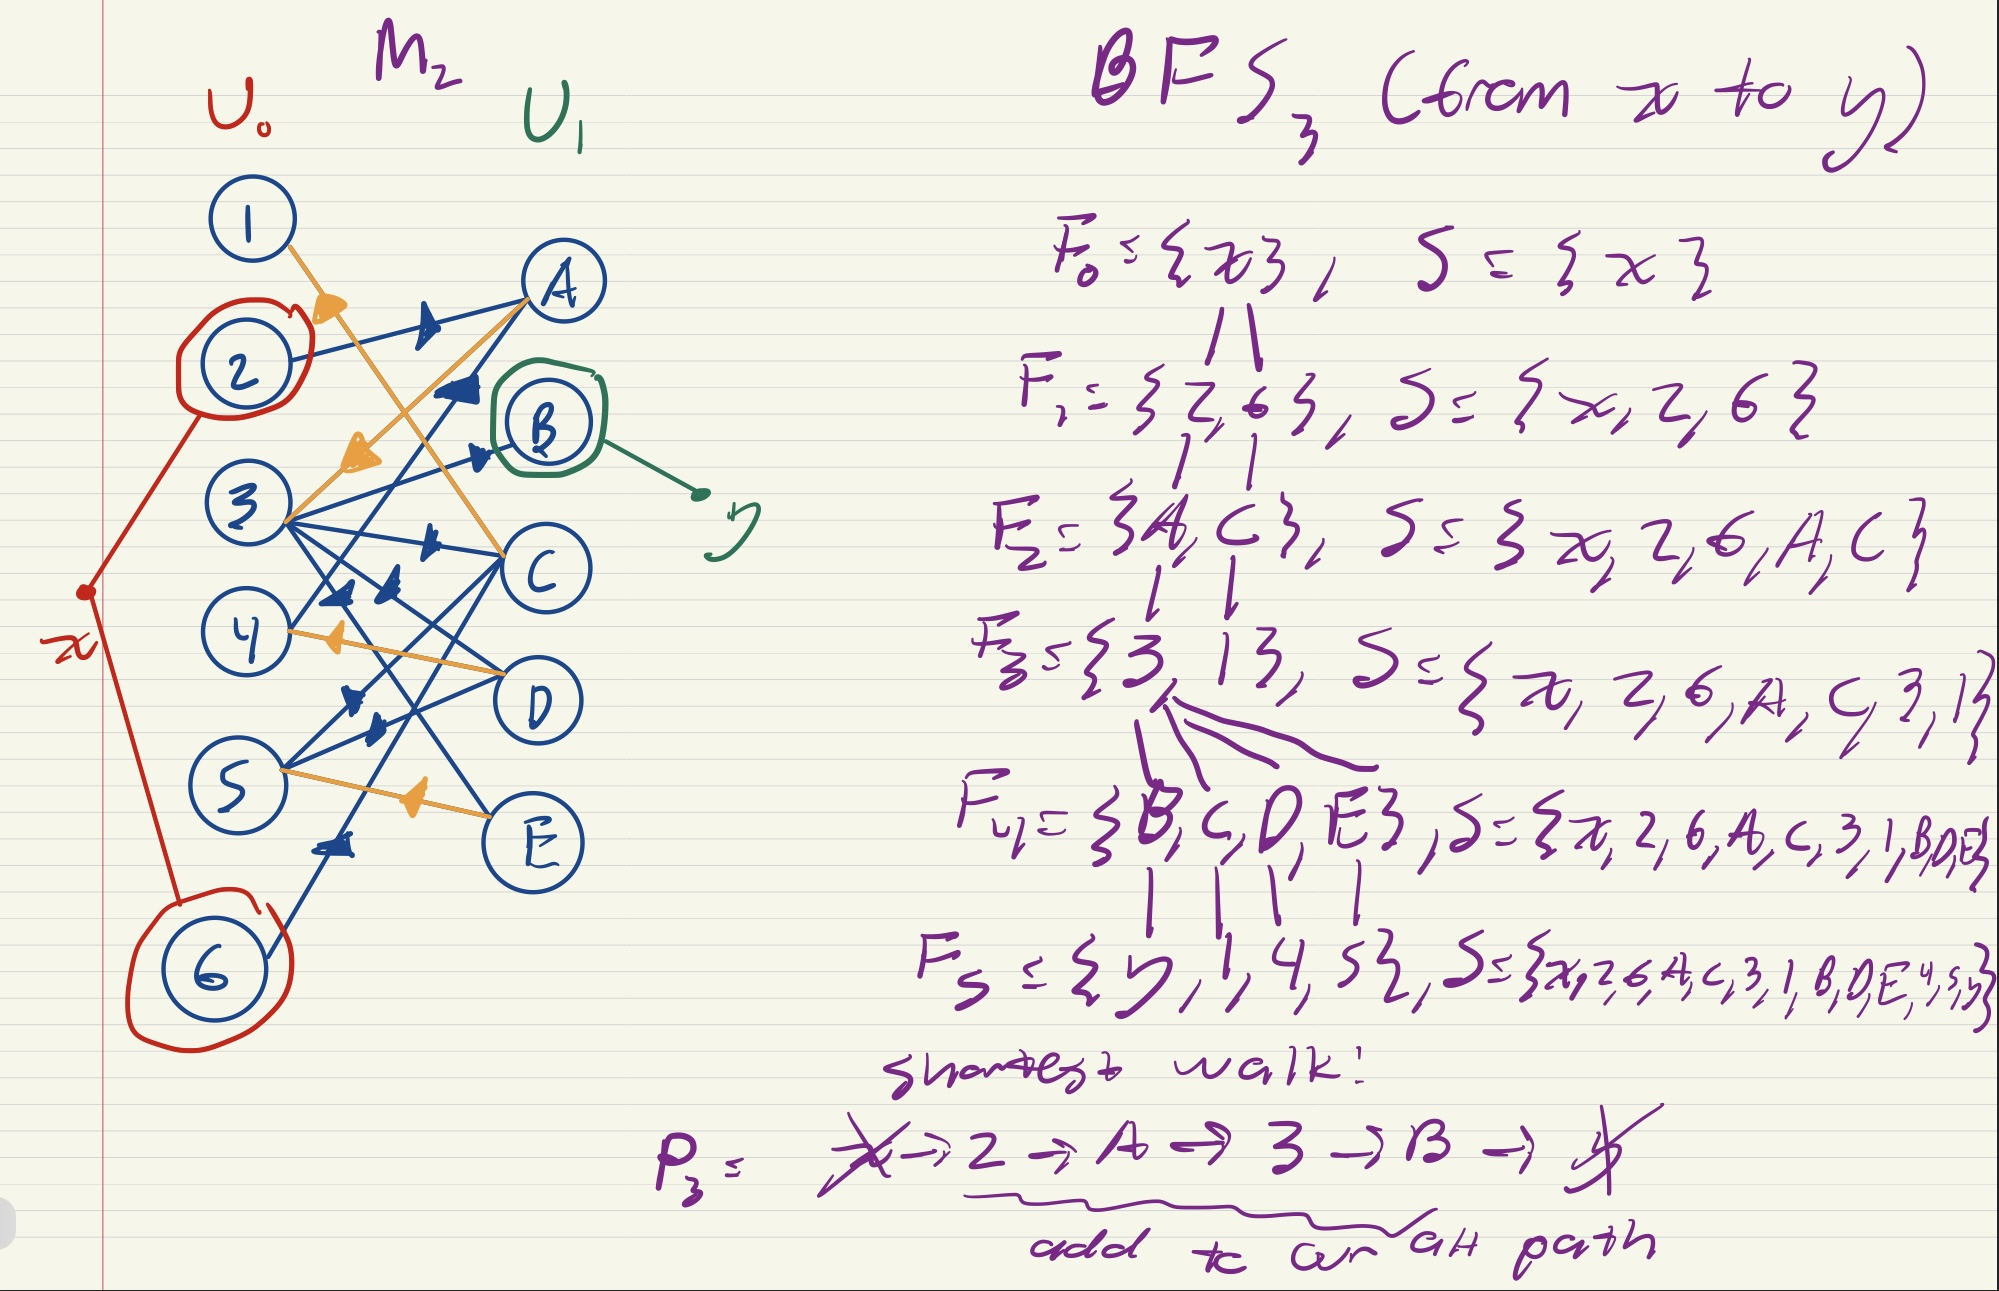
\includegraphics[width=0.75\linewidth]{IMG_0138.jpg}
    \caption{Next matching update, finding third shortestwalk}
    \label{fig:enter-label}
\end{figure}

\begin{figure}[H]
    \centering
    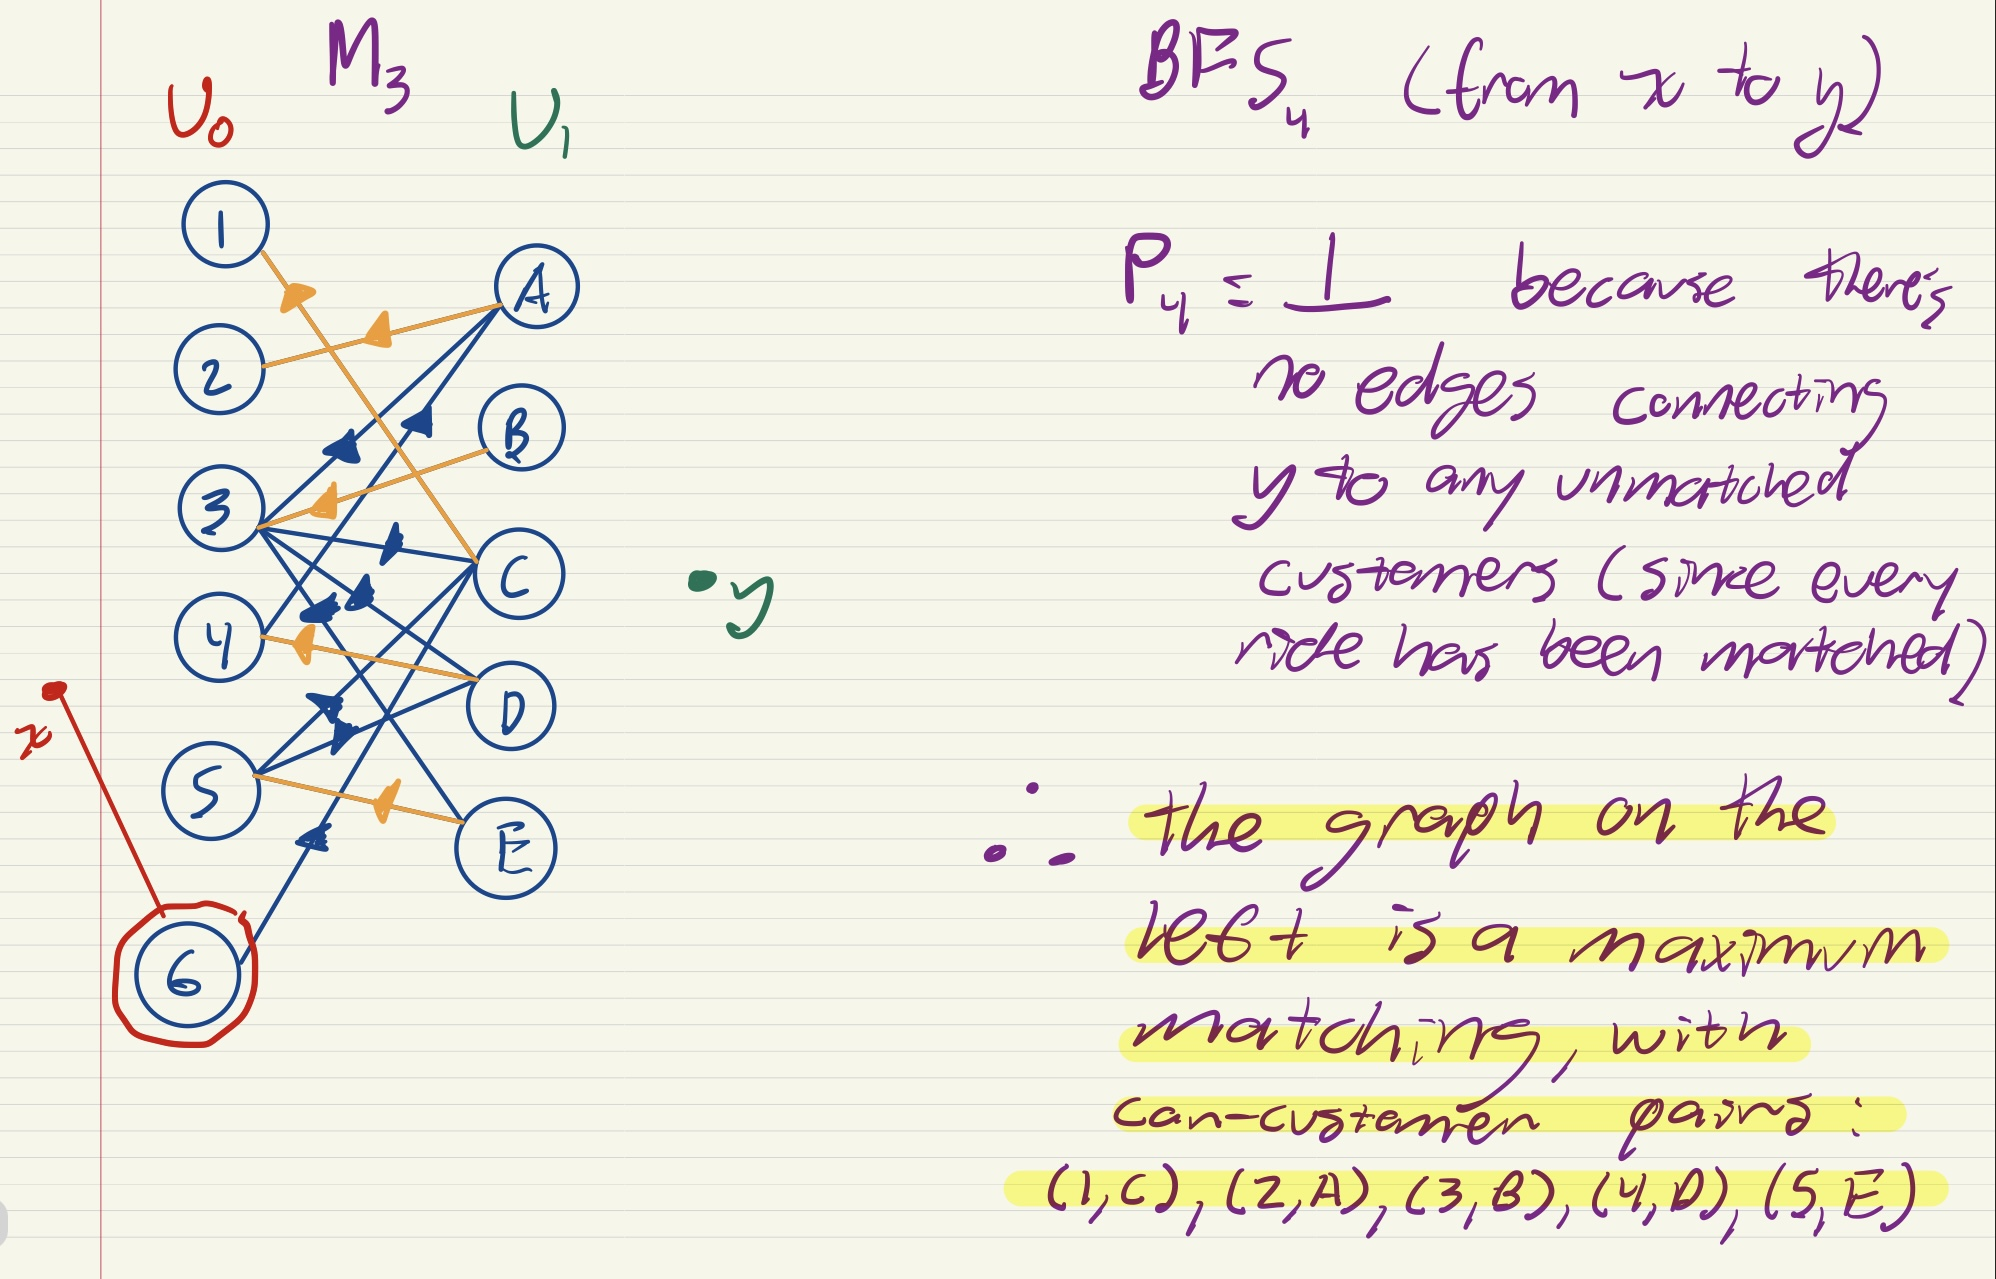
\includegraphics[width=0.75\linewidth]{IMG_0139.jpg}
    \caption{Final matching update (it's max size)}
    \label{fig:enter-label}
\end{figure}

        
    \end{enumerate}

    \item (Vertex-Weighted Matching)
        For a graph $G=(V,E)$ and a subset $F\subseteq E$, let $V(F)$ denote the set $\bigcup_{f \in F}f$ of vertices that are an endpoint of at least one edge in $F$.
        \begin{enumerate}
            \item Prove that if $G=(V,E)$ is a graph and $M\subseteq E$ is a matching in $G$, then there is a maximum-size matching $M'$ such that $V(M)\subseteq V(M')$.  (Hint: consider constructing a maximum matching via augmenting paths, but starting with $M_0=M$ rather than $M_0=\emptyset$. What can you say about the $V(M_i)$'s?) \label{part:monotonicity}\\

            Starting with our matching $M_0 = M$, I will show that there's a maximum matching $M'$ that we can construct such that $V(M)\subseteq V(M')$. I will prove this justifying a subclaim using the loop invariant, and using that subclaim to prove the main claim. \\
            
Here's some pseudocode for constructing $M'$ from $M_0$ using a while loop:

\begin{itemize}
    \item \textbf{While} there exists an augmenting path $P$ in the graph with respect to the edges in $M$:
    \begin{itemize}
        \item Increase the size of $M$ by swapping the matched and unmatched edges along $P$. \\
    \end{itemize} 
\end{itemize} 

            \textbf{SUBCLAIM} \\

            I will now prove the loop invariant holds by showing that for each $M_i$ where $i > 0$, $V(M_{i-1}) \subseteq V(M_i)$, which confirms that $V(M_0) \subseteq V(M')$ with $M'$ being $M_j$ for the $j$ that represents the maximum number of times we can increase our matching size. \\

            This proof is based on the fact that an augmenting path is an alternating walk that contains an alternating walk in the current $M_{i-1}$. It's basically that alternating walk in the current $M_{i-1}$, but with edges connecting the $v_0$ or $v_x$ in the original walk to new unmatched starting and ending vertices $v_0'$ or $v_x'$ in the augmented path. \\
            
            Swapping the matched and unmatched edges in $P$ ensures the vertices in the original alternating walk will be included in our increased size matching $M_i$ because it turns the augmented path into an alternating walk where the first and last edges traversed are included in the new $M_i$. No vertices reached in an original alternating walk wrt the edges in $M_{i-1}$ will be excluded from $V(M_i)$ because swapping the matched and unmatched edges in $P$ preserves the identity of that original alternating walk within $P$ as being an alternating walk. Adding new $v_0'$ or $v_x'$ to that path (which will respectively end up matched $v_0$ or $v_x$) confirms that the ${v_0, v_x} \in V(M_{i+1})$. Overall, that means the same vertices in $V(M_{i-1})$ will be present in $V(M_{i})$, as all that changes with the vertices in $V(M_{i-1})$ once we make $V(M_{i})$ are the identities of their neighbors in $M_i$. \\
            
            A simple example to illustrate is that if we had an alternating walk with $M_{i-1}$ in $G$ along edges [\textbf{(1,2)}, (2,3), \textbf{(3,4)}], with \textbf{bolded} edges being part of our matching, there may be an augmented path [(0,1), \textbf{(1,2)}, (2,3), \textbf{(3,4), (4,5)}] that we could alter through edge swapping to [\textbf{(0,1)}, (1,2), \textbf{(2,3)}, (3,4), \textbf{(4,5)}] with $M_i$ in $G$. We can clearly see that $\{ 1,2,3,4 \} \subseteq \{0,1,2,3,4,5\}$. Generally, $V(M_{i-1}) \subseteq V(M_i)$ since the vertices in all bolded edges in the alternating walk with $M_{i-1}$ in $G$ will be included in the set of vertices in all bolded edges in the alternating walk with $M_{i}$ in $G$. Thus, we've used the loop invariant to prove my claim that $V(M_{i-1}) \subseteq V(M_i)$. \\
            
            \textbf{MAIN CLAIM} \\

            I have so far proven via the loop invariant that $V(M_{i-1}) \subseteq V(M_i)$ for $i > 0$. Now, it's pretty easy to prove that $V(M)\subseteq V(M')$. We know by Berge's theorem that $v_0'$ and $v_x'$, the additional vertices that can be included in an alternating walk to form an augmenting path, only exist when there exists an augmenting path. When there isn't an augmenting path in $G$ wrt a current matching $M'$, that means $M'$ is a maximum sized matching. The algorithm above constructs $M'$ using $M_0 = M$ as a starting point, creating larger and larger matchings $M_i$ until we reach $M_j$ with $M_j = M'$ and $i \geq i$ (at which point there's no more augmenting paths in the graph, showing that $M'$ is a maximum sized matching by Berge's theorem). Since I've proved that each $V(M_{i-1}) \subseteq V(M_i)$ for $i > 0$, we therefore know that $V(M) \subseteq V(M_j) \Leftrightarrow V(M) \subseteq V(M')$. This follows from the fact that if $A \subseteq B, B \subseteq C \rightarrow A \subseteq C$ (so the vertices in our starting matching are a subset of the vertices in every matching of increasing size that we construct using augmenting paths). \\

            Also, it's good to address the trivial case in which $M = M_0 = M'$. By the definition of subset, $V(M') \subseteq V(M')$, so the claim holds even if we never end up iterating through the while loop (besides the intial check for existing augmented paths). \\
            
        \item   In the Embedded EthiCS module, we saw how simply maximizing the {\em size} of a matching may not always be the right objective.  Thus, it is natural to consider weighted versions of the matching problem. Suppose 
        we consider vertex-weighted graphs $G = (V,E,w)$, $w$ is an array specifying a nonnegative vertex weight $w(v)$ for every $v\in V$.  (For example, the weight assigned to a patient might correspond to the number of extra years of life they would gain from a donation.)
          The goal of the {\em vertex-weighted maximum matching problem} is to find a matching $M$ maximizing its {\em total weight} $$w(M) = \sum_{\{u,v\}\in M} (w(u)+w(v)).$$
        (This corresponds to the utilitarian objective discussed in Embedded EthiCS module.)
        Using Part~\ref{part:monotonicity}, prove that every graph $G$ has a matching $M^*$ that simultaneously maximizes both total weight and size.  That is, for every matching $M$ in $G$, we have
        both $w(M)\leq w(M^*)$ and $|M|\leq |M^*|$.

        This still leaves the question of whether there efficient algorithms to optimize vertex-weighted matching.  This problem can be reduced to the maximum-flow problem, which is covered in CS1240.\\


        I will prove that every graph $G$ has a matching $M^*$ that simultaneously maximizes both total weight and size. \\

        \textbf{Proof by Contradiction:} \\
        Assume, for contradiction, that there DOES NOT exist a matching $M^*$ in every graph $G$ that simultaneously maximizes both total weight and size. \\

        \textbf{Contradiction Argument:} \\
        This assumption allows for the existence of a matching, $\hat{M}$ which maximizes weight but not size at the same time. In other words, $w(M) \leq w(\hat{M})$ and $|\hat{M}| < |M'|$ (where $M$ is every matching in G and $M'$ is a maximum size matching). However, $\hat{M}$ can't possibly maximize weight without maximizing size. Since $\hat{M}$ isn't maximizing size, this means (by Berge's theorem) that there exists an augmenting path in G wrt the matching $\hat{M}$ which can be used to increase the size of the matching $\hat{M}$. Increasing the size of $\hat{M}$ to $\hat{M}_{larger}$ (i.e. adding in more edges) necessarily increases $w(\hat{M})$ to $w(\hat{M}_{larger})$. $w(\hat{M}_{larger}) > w(\hat{M})$ because of the addition of the positive weights of the extra vertices $v_0'$ and $v_x'$ (defined above in 3a) in $V(\hat{M}_{larger})$. Since we can find a matching with weight greater than $w(\hat{M})$ by increasing the size of $\hat{M}$ to $\hat{M}_{larger}$ (as $\hat{M}$ is not a maximum size matching), \textit{$\hat{M}$ doesn't actually maximize weight!} \\

        \textbf{Conclusion: } \\
        We've shown a matching $\hat{M}$ that maximizes weight but not size is not actually maximizing weight (because increasing the size would increase the weight). Our assumption, for contradiction, is what provides the notion of such a $\hat{M}$ existing in $G$. Thus, that assumption must be false, so we have proved the opposite of the assumption is true by contradiction: there DOES exist a matching $M^*$ in every graph $G$ that simultaneously maximizes both total weight and size. QED. \\

        \item (optional\footnote{This problem won't make a difference between N, L, R-, and R grades. As this problem is purely extra credit, course staff will deprioritize questions about this problem at office hours and on Ed.}) Show how to reduce matching with the {\em maximin} objective to vertex-weighted matching,\footnote{In lecture, Salil said that he did not know whether there were efficient algorithms to optimize the maximin objective, but afterwards we realized that this reduction allows it to be solved via maximum flow algorithms, as covered in CS1240.}
        and deduce that there is always a matching $M$ that simultaneously maximizes the maximin objective and $|M|$.  For simplicity, you may assume that there are no ties in how well off the patients are prior to treatment.  (Hint: use weights that are powers of 2.) \\

        This is easy money! To provide some context, the \textit{maximin} objective focuses on matching donors to patients by priority of which patients start out with the \textit{least} number of QUALYs.\\

        \textbf{REDUCTION} \\

        \textbf{Preprocessing:} \\
        We need to make a vertex-weighted graph. We can do this by creating our bipartite graph similarly to before, with donors/patients having no within-group edges and edges between donors and patients representing compatibility. However, each vertex shall have a weight attribute as well which can also be stored in an array $w$. Donors will ALL get their weight attributes assigned to zero since we only care about the patient health in the $maximin$ objective, and every patient $i$ will get their weight attribute assigned to $2^{-{QALYS}_i}$, where ${QALYS}_i$ is the number of quality-adjusted life years lived so far by patient $i$. \\

        \textbf{Oracle:} \\
        We shall run the oracle that solves the problem of finding a weight-maximizing matching in a vertex-weighted bipartite graph. \\

        \textbf{Postprocessing:} \\
        Not necessary, assuming the oracle returns us the set of edges in a weight-maximizing matching within our vertex-weighted bipartite graph of patients and their potential donors. \\

        \textbf{CORRECTNESS: }\\
        By assigning each patient $i$ a weight attribute equal to $2^{-QALYS_i}$, patients who've lived fewer QALYs will have higher weights. I put the "$-$" in the exponent to ensure that's the case. Thus, calling an oracle that finds the weight-maximizing matching in reality matches donors to patients who've lived the fewest QALYs. This results in our matching fitting the $maximin$ objective because patients with the fewest QALYs lived get priority in the matching process. \\

        \textbf{DEDUCTION:} \\
        I can deduce that there is always a matching $M$ that simultaneously maximizes the maximin objective and $|M|$ using the result of my proof from 3b: there DOES exist a matching $M^*$ in every graph $G$ that simultaneously maximizes both total weight and size. In the implementation of my reduction above, maximizing total weight in a matching is equivalent to maximizing the $maximin$ objective. Thus, there is always a matching $M$ that simultaneously maximizes the $maximin$ objective (via maximizing weight in my implementation) and size, making such an $M$ a matching of maximum size and impact according to Rawlsian economics. 

        

        

        
        
        \end{enumerate}

    \item (EthiCS Reflection) Suppose there are two patients in need of an immediate kidney transplant, but only one donor is currently available. The donor’s kidney is compatible with both patients. Patient A starts at 30 QALYs and is expected to live 3 additional QALYs as a result of the transplant. Patient B starts at 45 QALYs, and is expected to live 10 additional QALYs as a result of the transplant. {\em All else being equal}, \textbf{which patient should the kidney go to, and why?} Your response should take the form of a short paragraph (3-4 sentence) reflection. In explaining your ethical reasoning about the case, be sure to draw on at least one concept discussed in class.

    \textit{Note: As with the previous psets, you may include your answer in your PDF submission, but the answer should ultimately go into a separate Gradescope submission form.}

    \item Once you're done with this problem set, please fill out \href{https://forms.gle/4D5u71QSidk4VLoV9}{this survey} so that we can gather students' thoughts on the problem set, and the class in general. It's not required, but we really appreciate all responses!
    
\end{enumerate}

\end{document}